\documentclass[10pt]{article}
\usepackage[final]{pdfpages}
\usepackage{cleveref}
\usepackage{xparse}
\usepackage{hyperref}
\usepackage{geometry}
\usepackage{amsmath}
\usepackage{graphicx}
\usepackage{caption}
\usepackage{subcaption}
\usepackage[section]{placeins}
\usepackage{listings}
\usepackage{verbatim}
\usepackage{harvard}
\usepackage[dcucite,abbr]{harvard}
\usepackage{sectsty}
\usepackage{html}
\usepackage{url}
\sectionfont{\rmfamily\mdseries\Large}
\subsectionfont{\rmfamily\mdseries\itshape\large}


\geometry{
  %body={6.5in, 8.5in},
  left=2.5cm,
  right=2cm,
  top=2cm,
  bottom=2cm
}

\linespread{1.213}
\begin{document}
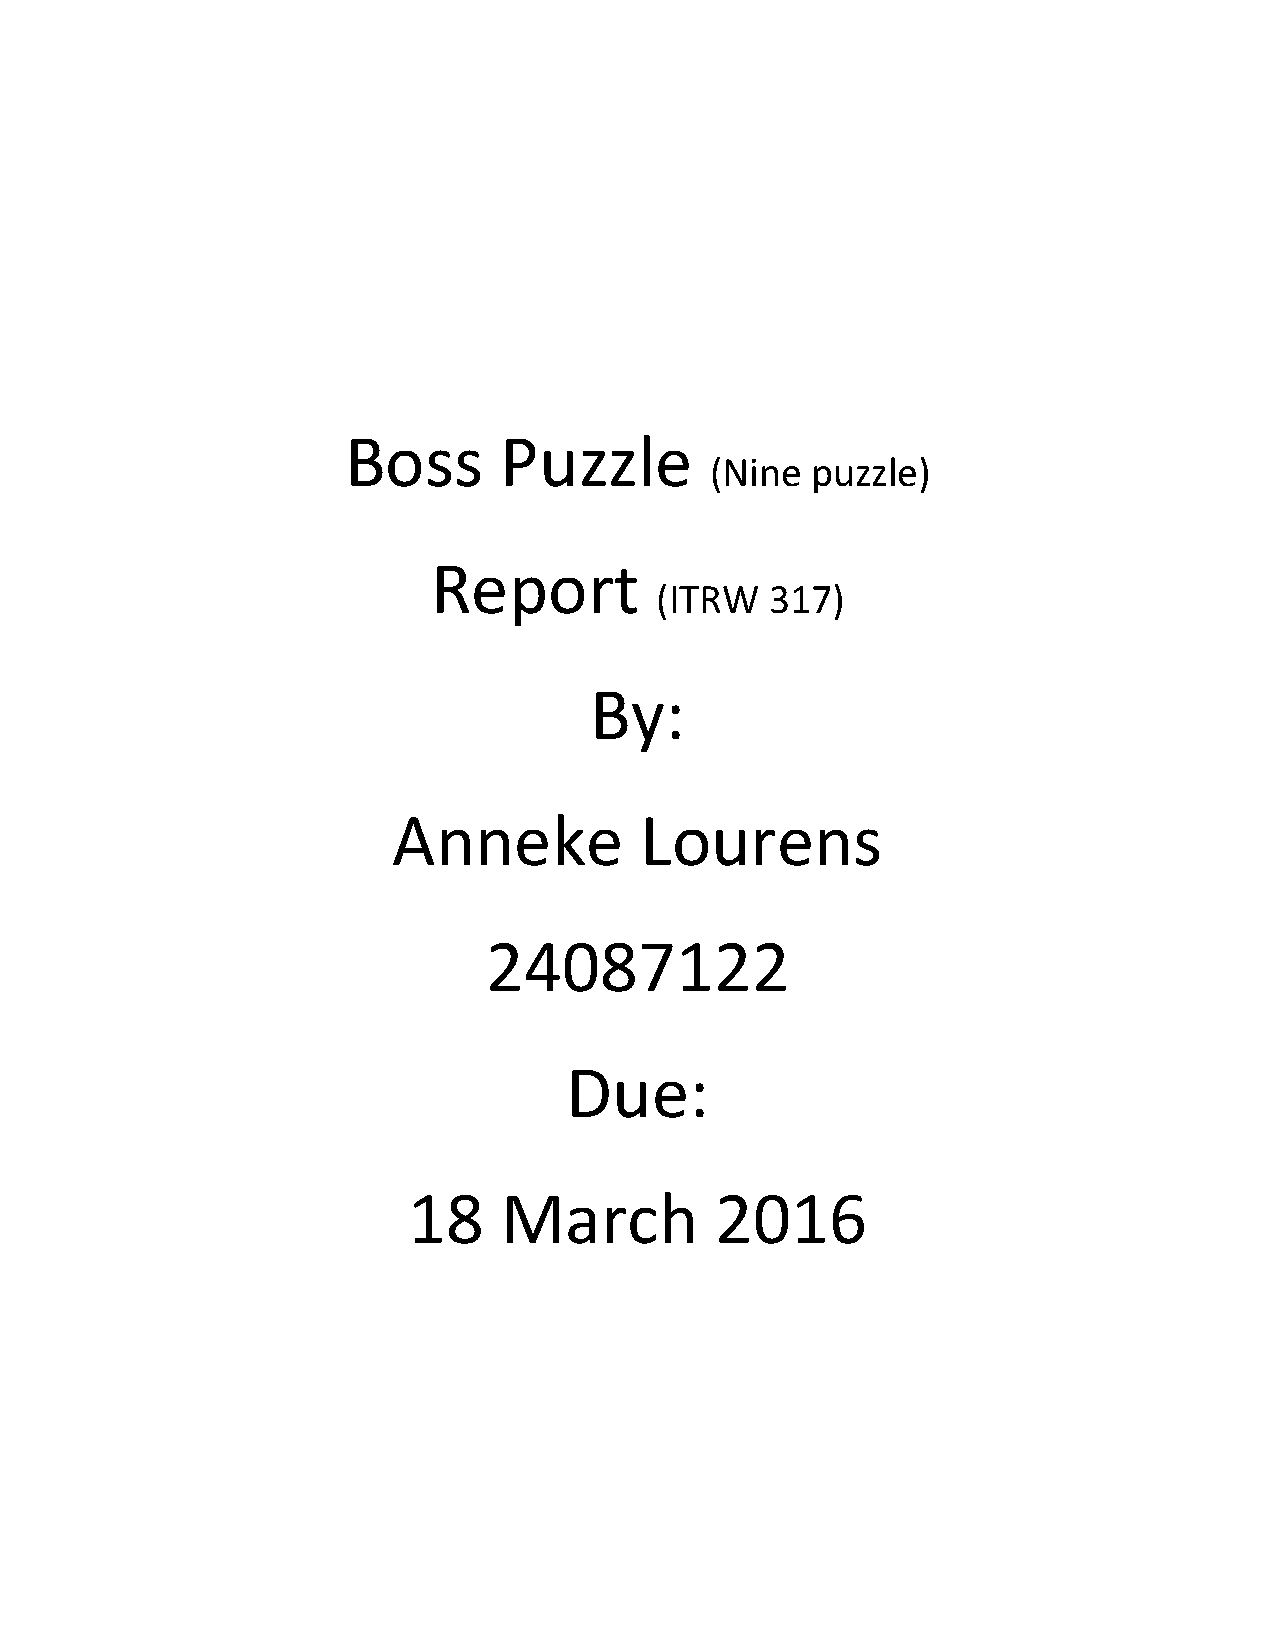
\includepdf{./BossPuzzle.pdf}
\newpage
\index{}
\newpage
\section*{Introduction}

\section*{Background}

\section*{History}

\section*{Literature Study}

\section*{User Guide}
\subsection*{How to begin the Nine-puzzle}
Step 1:
Right click on the execute.bat file and open it with notepad.
Change the name of the .csv file.  Save the file and exit it.  Double click on the file to run the file. Figure~\ref{beginfile}
\begin{figure}
\centering
 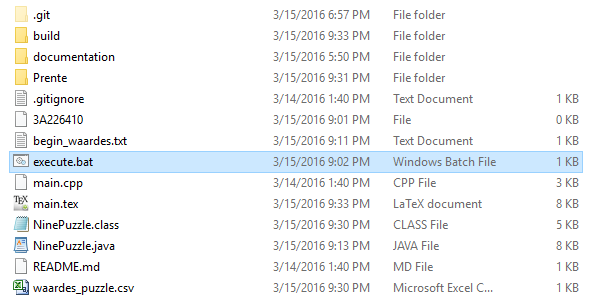
\includegraphics[scale=0.5]{./Prente/beginfile.png}
 \caption{}
 \label{beginfile}
\end{figure}
\\Step 2:
\begin{figure*}[b!]
    \centering
    \begin{subfigure}[b]{0.5\textwidth}
        \centering
        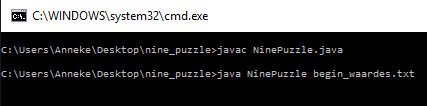
\includegraphics[scale=0.8]{./Prente/begincmd.png}
        \caption{if you have run the execute.bat file}
        \label{begincmd}
    \end{subfigure}%
 
    \begin{subfigure}[b]{0.5\textwidth}
        \centering
        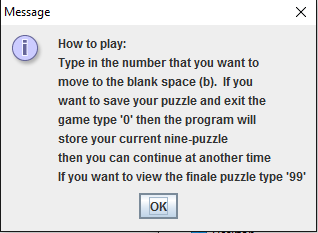
\includegraphics[scale=0.8]{./Prente/MessageBegin.png}
        \caption{The program will show this message directly after you have run the execute.bat file}
        \label{MessageBegin}
    \end{subfigure}
    \caption{\label{1}}
   \end{figure*}
If the program has run you will see figure Figure~\ref{1}
\\Step 3: Enter a y for you are a new player or n for you are not a new player Figure~\ref{prent1}
\begin{figure}
\centering
 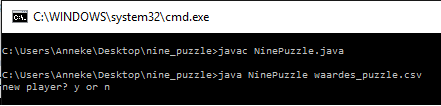
\includegraphics[scale=0.8]{./Prente/prent1.png}
  \caption{This figure asks if you are a new player or not}
  \label{prent1}
\end{figure}
\\Step 4:
\begin{figure}
\centering
 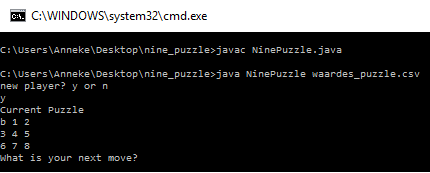
\includegraphics[scale=0.8]{./Prente/prent2.png}
 \caption{}
 \label{prent2}
\end{figure}
After step 3 is completed the begin puzzle will be given. Figure~\ref{prent2}
\\Step 5:
\begin{figure}
\centering
 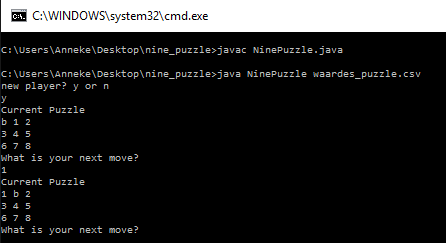
\includegraphics[scale=0.8]{./Prente/prent3.png}
 \caption{}
 \label{prent3}
\end{figure}
Enter the number that you want to move like in Figure~\ref{prent3}. The game will move that number to the blank space(b) and give the updated puzzle again.
\subsection*{Functionality}
How to stop save and exit the program:
If you want to stop playing and play again later then you can type 0 then the puzzle will be saved and the game will exit. Figure~\ref{2}
\begin{figure*}[b!]
    \centering
    \begin{subfigure}[b]{0.5\textwidth}
        \centering
        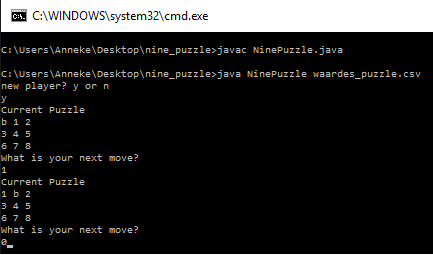
\includegraphics[scale=0.8]{./Prente/prent4.png}
        \caption{If you type in 0}
        \label{prent4}
    \end{subfigure}%
 
    \begin{subfigure}[b]{0.5\textwidth}
        \centering
        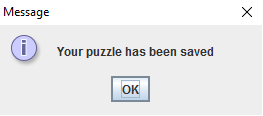
\includegraphics[scale=0.8]{./Prente/prent5.png}
        \caption{The message will show that you work has been saved}
        \label{prent5}
    \end{subfigure}
    \caption{\label{2}}
   \end{figure*}
   
If you have won the game the program will save your work and show a message to congratulate you and show how many moves you have made to solve the puzzle. Figure~\ref{prent6} 
\begin{figure}
\centering
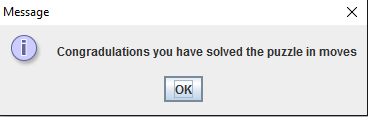
\includegraphics[scale=0.8]{./Prente/prent6.png}
\caption{}
\label{prent6}
\end{figure}

If you want to view the finale puzzle you type in 99. Figure~\ref{prent7}
\begin{figure}
\centering
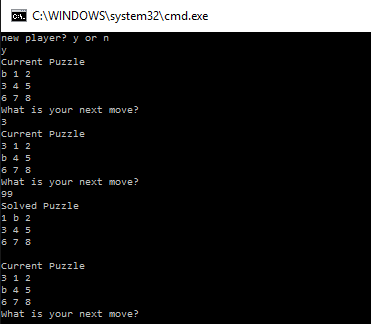
\includegraphics[scale=0.8]{./Prente/prent7.png}
\caption{}
\label{prent7}
\end{figure}

\section*{Code}
 \begin{tiny}
  \begin{verbatim}
import java.util.Scanner;
import java.io.File;
import java.io.FileNotFoundException;
import java.io.FileReader;
import java.io.IOException;
import java.io.PrintWriter;
import javax.swing.JOptionPane;

public class NinePuzzle {  
  public static void main(String[] args) throws FileNotFoundException {
    // scanner to read out of txt file
    Scanner input = new Scanner(args[0]);
    // gebruiker se skuiwe
    Scanner gebruiker = new Scanner(System.in);
    boolean solved = false;
    boolean save = false;
    int count = 0;
    // create arrays
    int[] current = new int[9];
    int[] finaal = new int[9];
    // array for the string read in csv file
    String[] userInputs = new String[1];
    String filename = input.nextLine();
    // call method that reads the csv file
    setUpArray(current, finaal, userInputs, filename);  
    // display how the game is played
    String message = "How to play: \n" +
	                 "Type in the number that you want to \n" +
                     "move to the blank space (b).  If you \n"+
					 "want to save your puzzle and exit the \n"+
					 "game type '0' then the program will \n"+
					 "store your current nine-puzzle \n" +
                     "then you can continue at another time \n"+
					 "If you want to view the finale puzzle type '99'";
    JOptionPane.showMessageDialog(null, message);
    // while loop to see if the user has finished playing
	System.out.println("new player? y or n");
	String newUser = gebruiker.nextLine();
	String yn = newUser.substring(0, 1);
	if (yn.equals("y") ||  yn.equals("Y")) {
	  userInputs[0] = "";
      writeArrayToFile(current, finaal, userInputs[0], filename);
	}
    while ( !solved && !save) {
      System.out.println("Current Puzzle");
      puzzle(current); // print current puzzle
      int lees = 0;
      // ask user what his next move is going to be
      System.out.println("What is your next move?");
      lees = gebruiker.nextInt();
      // test if the input from user is 0 or any other number between 1 - 8
      if ( lees != 0 ) {
        if(lees == 99) {
          System.out.println("Solved Puzzle");
          puzzle(finaal);
          System.out.println("");
          } else {
          // move the index of the tiles
          move_index(lees, current);
          count++;
          solved = compare_solution(finaal, current);
          userInputs[0] += Integer.toString(lees) + ",";
          }  
      } else { //if the user enters 0
        //write current puzzle to csv file
        writeArrayToFile(current, finaal, userInputs[0], filename);
        //stoor na txt file as begin waardes
        save = true;
      }//end if
      //show the final puzzle to the user        
    }// end while  
    // show message that say he has solved  the puzzle
    if ( solved ) {
      String message1 = "Congradulations you have solved the puzzle in moves";
      JOptionPane.showMessageDialog(null, message1);
      System.out.println("jy het" + " " + count + " " 
      + "skuiwe gemaak om die puzzle klaar te maak");
    }
	if(save){
	  String message2 = "Your puzzle has been saved";
      JOptionPane.showMessageDialog(null, message2);
	}
}//end main
  
  public static void writeArrayToFile(int [] current,
                                       int [] finaal,
                                    String userinputs,
                                    String filename) 
                  throws FileNotFoundException {
    try {
      PrintWriter outputStream = new PrintWriter(filename);
      for ( int k = 0; k < 9; k++ ) {
        if ( k != 8 ) {
       // write the current puzzle to file
          if(current[k] == 0) {
            outputStream.print("b,");
          } else {  
            outputStream.print(current[k] + ","); 
          }
        } else {
            outputStream.print(current[k] + "\r\n");
        }
      }
    for(int h = 0; h < 9; h++ ) {
      if (h != 8) {
        if (finaal[h] == 0) {
          outputStream.print("b,"); 
        } else {
            outputStream.print(finaal[h] + ",");
        }
      } else {
        outputStream.print(finaal[h] + "\r\n");
      }//end else
    }    
    if (userinputs.length() > 0) {
      String user_inputs = userinputs.substring(0, userinputs.length() - 1) + "\r\n";
      outputStream.println(user_inputs);
    }
    outputStream.close();
    } catch (FileNotFoundException e) {
        e.printStackTrace();
    }//end catch
  }
  //read csv file into an array
  public static void setUpArray(int [] current, int [] finaal, String [] userinputs, String filename) throws FileNotFoundException {
    File File = new File(filename);  
    try {
      Scanner inputStream = new Scanner(File);
      int lines_read = 0;
      while (inputStream.hasNext() ) {
        String data = inputStream.next();//gets a whole line
        String [] values = data.split(",");
        if ( lines_read == 0 ) {
          for ( int v = 0; v < 9; v++ ) {
            if (values[v].equals("b")) {
              current[v] = 0;
            } else {
              current[v] = Integer.parseInt(values[v]); 
            }
          }
        } else if ( lines_read == 1 ) {
                 for ( int w = 0; w < 9; w++ ) {
                   if (values[w].equals("b")) {
                     finaal[w] = 0;
                   } else {
                       finaal[w] = Integer.parseInt(values[w]);
                   }
                 } 
        } else if ( lines_read == 2 ) {
		         if (!data.equals(null) || !data.equals("")) {
                   userinputs[0] = data + ",";
		         } else {
		             userinputs[0] = "";
		         }
        }
      lines_read++;  
    }
      inputStream.close();
    }
    catch(FileNotFoundException e) {
      e.printStackTrace();
    }      
  }//end setuparray
  //print puzzle
  public static int puzzle(int [] current) {
    for(int k = 0; k < 9; k++) {   
      if (current[k] == 0) {
        System.out.print("b ");
      } else {
          System.out.print(current[k] +" ");  
      }
      if ( ((k + 1) % 3) == 0 ) {
        System.out.print("\n");
      }
    }//end for
    return 0;
  }//end puzzle
  
  //swap the index of the tile that has been moved
  public static boolean move_index(int lees, int [] current) {
    int[][] lookup = {{1, 3, -1, -1},
                      {0, 2, 4, -1},
                      {1, 5, -1, -1},
                      {0, 4, 6, -1},
                      {1, 3, 5, 7},
                      {2, 4, 8, -1},
                      {3, 7, -1, -1},
                      {4, 6, 8, -1},
                      {5, 7, -1, -1}};
    int zero_position = get_index(0, current);
    int value_position = get_index(lees, current);
    for ( int i = 0; i < 4; i++) {
      if ( lookup[zero_position][i] == value_position ) {
        current[value_position] = 0;
        current[zero_position] = lees;
    return true;
      }
    }
  return false;
  }//end move_index
  //get the index of the blank space and the number that the user want to move
  public static int get_index(int lees, int [] current) {
    for ( int i = 0; i < 9; i++ ) {
      if ( lees == current[i] ) {
        return i;
      }
    }
  return 0;
  }
  //compare wether the current puzzle has the same values of the final puzzle
  public static boolean compare_solution(int [] finaal, int [] current) {
    for ( int i = 0; i < 9; i++) {
      if ( finaal[i] != current[i] ) {
        return false;
      }
    }
    return true;
  }//end compare
}//end class
  \end{verbatim}
   \end{tiny}
   \section*{Bibliography}
\bibliographystyle{dcu}
\bibliography{BIBTEXFILE}
\end{document}